% !TEX root = ../tjumain.tex
\chapter{协议实现部分}

首先,从宏观上阐释:我们TCP实现部分采用了两个线程进行服务:发送线程和接收线程。

\paragraph*{发送线程} 负责从数据结构 sending\_queue 中取出并按需发送报文、设置时钟,检查时钟进行超时重传。在用户调用 tju\_socket 生成 socket 时创建。首先发送线程会到达 ACK 时预订消除的时钟进行 删除,然后判断是否有超时时钟,执行重传。最后进行正常报文的发送。

\paragraph*{接收线程} 负责从socket中获取对方发送的报文、返回 ACK 并处理不按需到达的报文,确保放入 recv\_buf 中的数据是正确且有序的。在接收线程收到包裹后,调用 tju\_handle\_packet 进行处理。

\paragraph*{tju\_handle\_packet} 处理报文的主要函数,通过 switch ,根据当前 socket 的状态选择合适分支进行报文的处理。

\section{连接建立的实现}

要实现连接的建立,我们实现了如图\ref{fig:established}的流程图。实现了 tju\_conn 和 tju\_accept 供 client 以及 server 端进行调用的 API

\paragraph*{tju\_conn} Client 端通过该 API 对Server 端发起连接请求。而后进入等待循环,直到自己 socket 的状态变为 Established 再返回。而 socket 状态的改变则由接收线程处理。

\paragraph*{tju\_accept} Server 端调用该API,从处于 LISTEN 状态的 socket 的 full\_connection 列表中获取一个全连接的 socket 即可。

\paragraph*{接收线程-三次握手}在 tju\_handle\_packet 中,关于连接建立有如下三种情况:

\begin{enumerate}
    \item LISTEN: 此状态为 Server 端。接收到 SYN 报文后,Server 端将状态变为 SYN\_RECV 并发出 SYN | ACK 报文,同时将其放入半连接队列中,发送线程需要对半连接中的sock进行重发
    \item SYN\_SENT:此状态为 Client 刚发送完 SYN 包裹,从连接的角度来说是 Client 端。此时收到包裹应为 SYN | ACK,否则拒收,由发送线程进行重发。接收正确报文后,socket 状态调整为 ESTABLISHED,同时返回一个 ACK 报文答复。
    \item SYN\_RECV:此状态为 Server 端发送完 SYN | ACK 报文,等待client的ACK。得到 ACK 后,将其半连接的sock拿出,放入全连接队列,等待 tju\_accept 进行调用。
\end{enumerate}

\section{可靠数据传输的实现}

\subsection{数据结构}

为了更好地实现可靠数据传输,我们额外实现了三种数据结构进行更优化的处理。分别是 timer\_list,queue和tree。

\paragraph*{timer\_list} 是对超时重发的处理,本质上是一个队列,其实现的头文件如图\ref{fig:timer_list}所示。对于每个 timer 我们记录了它创建的时间和创建时根据 socket RTO 计算出的 timeout 时间,以及它所代表的 tju\_packet\_t 和重传时的回调函数。我们采用 list 链表的形式进行整个线性表的遍历。当然,我们需要对其进行加锁,避免出错。

\begin{figure}[!htbp]
    \centering
    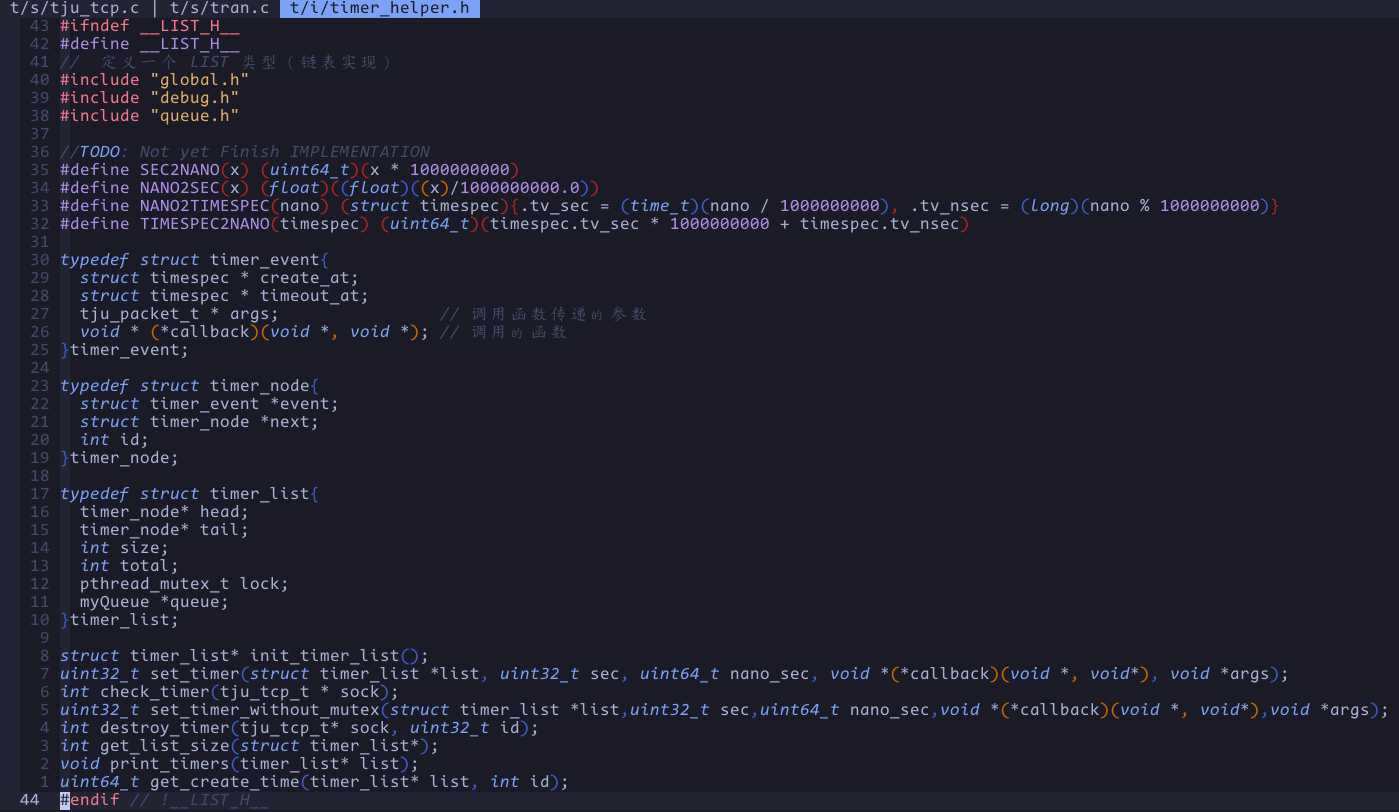
\includegraphics[width=1.0\textwidth]{timer_list.png}
    \label{fig:timer_list}\caption{timer\_list 数据结构}
  \end{figure}

\paragraph*{queue} 是对包括发送缓冲区、全连接队列以及清除队列(异步清除 timer )的具体实现。头文件如图\ref{fig:queue}所示。可以看到,我们使用 void* 表示当前结点装载的数据,这样实现的好处就是高扩展性,能够用来装载任何自定义的数据结构。缺点当然是使用不当会导致调用队列错乱。

\begin{figure}[!htbp]
    \centering
    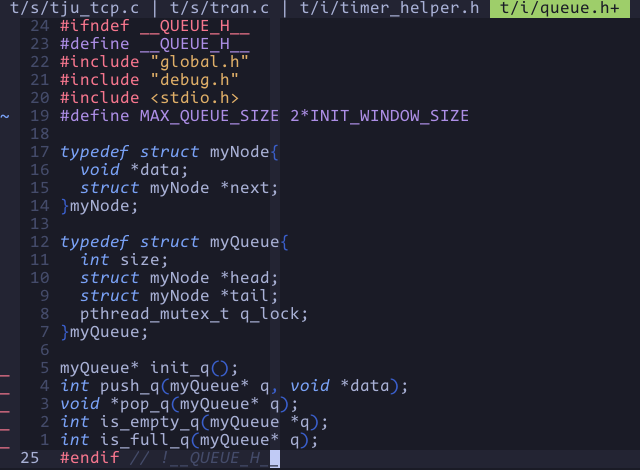
\includegraphics[width=0.9\textwidth]{queue.png}
    \label{fig:queue}\caption{queue 数据结构头文件}
  \end{figure}

  \begin{figure}[!htbp]
    \centering
    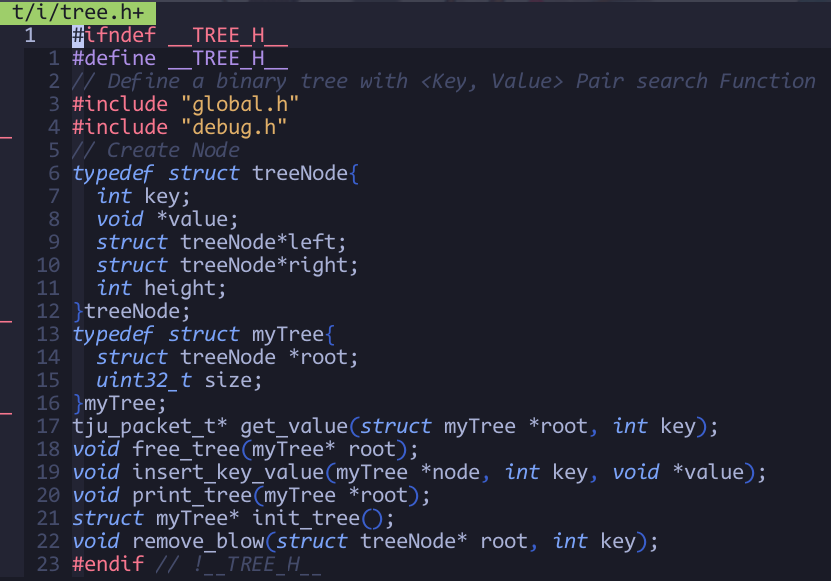
\includegraphics[width=0.9\textwidth]{tree.png}
    \label{fig:tree}\caption{tree 数据结构头文件}
  \end{figure}
  
\paragraph*{tree} 是对接收缓冲区的具体实现,在此我们采用了 AVL 的数据结构(自平衡搜索二叉树,aka 小根堆)。因为我们的应用场景是:存入乱序到达的包裹,并按照正序进行取出。使用 AVL 可将二者的操作时间复杂度降到 $log_2(N)$。图\ref{fig:tree}是 tree 的头文件。

\subsection{实现思想}

可靠数据传输的实现较为复杂。首先我们从发送线程的角度考虑,需要对发送的每个报文进行超时超时重传的检测。同时在接收到 ACK 后需要累计地将这些超时重传标签丢掉。

首先是在调用 tju\_send 时,按照原来的做法,是使用 send\_buf 进行发送。我们考虑到这个调用的流程逻辑本质上就是一种队列的思想:先从 tju\_send 进入发送队列的报文先发送。于是我们复用了半/全连接队列时创建的 QUEUE 数据结构,让 tju\_send 将报文放入 sending\_queue 中。再让发送线程通过 sending\_queue 取出需要发送的报文即可。

然后我们来处理超时重传:建立一个 timer\_list 结构,用于存放已经发送且未得到ACK的报文。在发送线程中,我们首先对这个 timer\_list 进行检查:按照顺序依次检查每个报文创建的时间和当前时间对比,如果有超时,则进行重发,否则直接退出。由于这个 timer\_list 特性,天然按照报文创建的时间进行排序,所以可以在第一次遇到不用重发时退出。

然后我们从接收写成的角度进行考虑:我们会接收到三种类型的报文:seq 小于、等于以及大于expected\_seq。所以我们的思路也就很明朗了:小于时将其丢弃,大于时将其放入之前定义的AVL树中,等于时将其放入 recv\_buf 并更新 expected\_seq,并在 AVL 树中按照 seq 的大小查找是否有乱序达到的报文。当然,三种情况都需要发送 ACK 回去通知收到。

\subsection{具体实现}

\paragraph*{Tju\_Send 实现} 在 Tju\_Send 中,首先需要判断上层内容的大小,若过大,则需要进行切片,以免在下层被切割。然后在进入阻塞状态,等待发送窗口出现空闲。然后交给发送窗口,同时调用发送函数,在 rwnd 的情况下将发送缓冲区的内容进行发送(此处在后期需要调整为 线程)

\paragraph*{Tju\_Recv 实现} 在 Tju\_Recv 中,首先进行阻塞等待,直到其他线程给接收缓冲区放入内容。待有内容后,再将内容 通过 Memcpy 提交给上层调用的实体。

\paragraph*{Socket 数据结构}
\begin{itemize}
    \item 给 window.wnd\_send 增加了 rwnd 和 cwnd 等控制发送的信息
    \item 给 window.wnd\_recv 增加了 AVL Tree 等数据结构,用于存放乱序到达的数据包
    \item 给 window.wnd\_send 增加了 rto 等字段,动态控制超时事件
    \item 给 window.wnd\_recv 增加了 expe\_seq 等字段,判断接收到的数据顺序正确与否
\end{itemize}

\subsubsection*{超时重传机制}

\paragraph*{超时重传定时器}
实现了 Timer\_Helpher 子系统,通过设置 set\_timer() 函数来新建一个 Timer,Delete\_timer() 来终止一个 Timer。使用了一个线程不断检查是否有超时的Timer,并进行重传和重置。使用 Mutex Lock 进行存储区域的一致性,使得在增加、删除和检查时只能有一个线程存在。

特别的,我们使用了链表的数据结构进行 Timer 的增加、删除和检查,链表能够高效地进行增加删除。同时,设置了 event 数据类型来处理当前 Timer 的超时操作(可以通过传入不同的函数和变量达到不同类型 Timer 的统一调用)。

\paragraph*{RTO调整}

由于我们每个需要重传的报文都对应一个 TIMER,所以我们能通过发送时的 Created\_At 和删除时的系统事件算出当前 Timer 提供的 sampleRTT 并 在每次进行 Timer 删除时,通过公式 \ref{eq:rto} 进行 RTO 的更新。

值得注意的是,这里依然需要大量使用 Mutex Locker 来控制:在更新 RTO 时,不能创建新的Timer,直到 RTO 更新完成。

\section{流量控制}

接收方发送ACK时,将自己缓冲区大小放入 advertised\_wind 字段。发送方在接收到 ACK 时,需要提取 rwnd 值。在设置发送窗口的大小时,我们需要考虑 rwnd(发送窗口大小), cwnd(拥塞控制), 以及自己本身的大小。

当得到 rwnd == 0 的情况时,发送方需要发送1比特的试探报文进行发送窗口的试探,同时需要设置超时机制进行不断试探。

\section{连接关闭的实现}

在实现连接关闭之前,我们需要统一说明一下目前 tju\_handle\_packet 中的 socket 状态种类,以便在后续的流程中解释更加清晰。

\paragraph*{连接建立} LISTEN, SYN\_SENT, SYN\_RECV, ESTABLISHED
\paragraph*{连接关闭} FIN\_WAIT\_1, FIN\_WAINT\_2, CLOSE\_WAIT, CLOSING, LAST\_ACK, TIME\_WAIT 

从代码实现的角度考虑,我们不需要在意当前情况是两方同时发起关闭还是一方先一方后。我们根据绘制的 FSM 图可以得出结论:我们根据 socket 状态以及接收到的报文进行状态的转换以及处理:

\begin{enumerate}
    \item \textbf{处于 ESTABLISHED 且发起 close} 发送 FIN 状态转化为 FIN\_WAIT\_1
    \item \textbf{处于 FIN\_WATI\_1 且收到 FIN 的 ACK} 状态转化为 TIME\_WAIT 超时后变为 CLOSED
    \item \textbf{处于 ESTABLISHED 收到 FIN} 状态变为 CLOSE\_WAIT 并返回 ACK 
    \item \textbf{处于 CLOSE\_WAIT 且发起 close} 状态转为 LAST\_ACK 且等待 ACK 
    \item \textbf{处于 LAST\_ACK 且收到 ACK} 状态转为 CLOSED 并关闭
\end{enumerate}

实现时需要注意的是,只要 socket 状态不是 CLOSED,都要继续接收新的报文并回复 ACK。

\section{拥塞控制的实现}

拥塞控制的实现核心在于两个事件触发拥塞窗口进行变化,且发送窗口随之而变。两个事件分别是:3个ACK,以及超时重传。

\paragraph*{3个ACK检测} 在 sock 中的 cwnd 数据结构中加入 last\_ack 以及 count 的整型数据,在 received\_ack 函数中对 last\_ack 进行比对并记录 count 是否增加或还原。

\paragraph*{超时检测} 在 check\_timer 中触发超时转换 cwnd 的大小。

需要注意的是需要创建一个 sshresh 对cwnd慢启动和拥塞避免进行转换。同时,需要记得在 3个ack后将状态调整为拥塞避免,在超时后将状态矫正为慢启动。


\section*{日志记录}

实现了日志 trace 模块,在Server Client 端调用 tju\_sock 的时候进行日志的初始化(即定义日志名,创建日志文件等)。然后通过提供的日志格式和事件,在相应事件发生时,调用响应函数进行日志的录入。



